\subsection{Dry run test-case}

A part with medium complexity is run through the algorithm to evaluate its validity (Table \ref{table_DryRun}).

\begin{table}[htb] % longtable does not work inside Table block
\caption{Step by step creation of Midsurface}
\begin{tabular}{@{}p{0.2\linewidth}  p{0.2\linewidth}  p{0.4\linewidth}  p{0.2\linewidth}@{}}
\toprule
Feature & Model & Midsurf Rule & Midsurface\\
\midrule
%------------------------------------------------------------------------------------------------------------------------------------
Sketch: Rectangle &

\raisebox{-0.9\height}{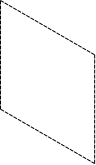
\includegraphics[width=0.6\linewidth]{..//Common/images//DryRun1.png}}

  &
For non-thin profile like this, no mid-curve. But for thin profile, it is computed&
\\
%-------------------------------------------------------------------------------------------------------------------------------------- 
Sketch: Add Circle as inner loop &
\raisebox{-0.9\height}{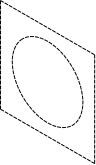
\includegraphics[width=0.6\linewidth]{..//Common/images//DryRun2.png}} &
For non-thin profile, no mid-curve. If the loop had made thin profile, mid-curves would be computed &
\\
%-------------------------------------------------------------------------------------------------------------------------------------- 
Face-Wall-Extrude (profile, thickness) &
\raisebox{-0.9\height}{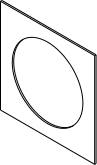
\includegraphics[width=0.6\linewidth]{..//Common/images//DryRun3.png}} &
For non-thin profile, Offset by 0.5*thickness. For thin, extrude midcurves by thickness. &
\raisebox{-0.9\height}{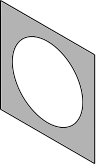
\includegraphics[width=0.6\linewidth]{..//Common/images//DryRun31.png}} \\

%-------------------------------------------------------------------------------------------------------------------------------------- 
Flange (edge, distance, angle)  &
\raisebox{-0.9\height}{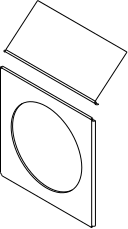
\includegraphics[width=0.6\linewidth]{..//Common/images//DryRun4.png}} &
Create Midsurface of the tool body. Extend-Trim to join to the existing Midsurface. &
\raisebox{-0.9\height}{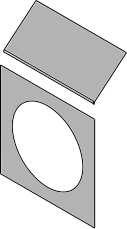
\includegraphics[width=0.6\linewidth]{..//Common/images//DryRun41.png}} \\

%-------------------------------------------------------------------------------------------------------------------------------------- 
Similarly add other Flanges  &
\raisebox{-0.9\height}{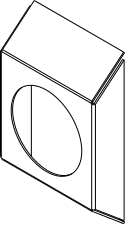
\includegraphics[width=0.6\linewidth]{..//Common/images//DryRun5.png}} &
Similarly join other tool-Mid-surfaces &
\raisebox{-0.9\height}{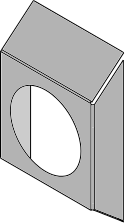
\includegraphics[width=0.6\linewidth]{..//Common/images//DryRun51.png}} \\
%-------------------------------------------------------------------------------------------------------------------------------------- 
Booleans  &
\raisebox{-0.9\height}{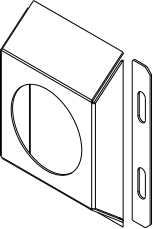
\includegraphics[width=0.6\linewidth]{..//Common/images//DryRun6.png}} &
Midsurfaces from tool and target bodies are extended-trimmed to join &
\raisebox{-0.9\height}{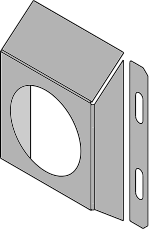
\includegraphics[width=0.6\linewidth]{..//Common/images//DryRun61.png}} \\

%-------------------------------------------------------------------------------------------------------------------------------------- 
Similarly add other Flanges  &
\raisebox{-0.9\height}{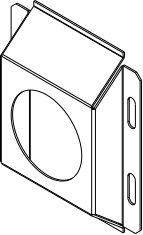
\includegraphics[width=0.6\linewidth]{..//Common/images//DryRun7.png}} &
Similarly join other tool-Mid-surfaces &
\raisebox{-0.9\height}{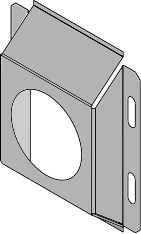
\includegraphics[width=0.6\linewidth]{..//Common/images//DryRun71.png}} \\

%-------------------------------------------------------------------------------------------------------------------------------------- 
Add small holes &
\raisebox{-0.9\height}{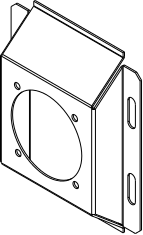
\includegraphics[width=0.6\linewidth]{..//Common/images//DryRun8.png}} &
No change in Midsurface as small holes are ignorable for Model Simplification. &
\raisebox{-0.9\height}{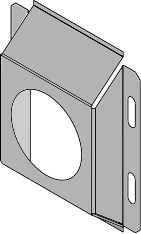
\includegraphics[width=0.6\linewidth]{..//Common/images//DryRun81.png}}\\
\bottomrule
%-------------------------------------------------------------------------------------------------------------------------------------- 
%\end{longtable}
\end{tabular}
\label{table_DryRun}
\end{table}

%\twocolumn % long table does not work in two-column mode, resetting back

%\end{table}